\documentclass[11pt,a4paper]{article}

% ---------------------------------------------------------------------------
% Compatibility of competing biochemical modules:
% capacity, recovery, and finite operation.
%
% Author metadata: set the macros below before submission.  They are
% deliberately left blank in this version.
% ---------------------------------------------------------------------------
\newcommand{\PaperAuthor}{}
\newcommand{\PaperAffiliation}{}
\newcommand{\PaperDate}{19 September 2026}

\usepackage[T1]{fontenc}
\usepackage[utf8]{inputenc}
\usepackage{lmodern}
\usepackage{microtype}
\usepackage[a4paper,margin=1.05in]{geometry}
\usepackage{amsmath,amssymb,amsthm,mathtools}
\usepackage{booktabs}
\usepackage{array}
\usepackage{enumitem}
\usepackage{xcolor}
\usepackage{graphicx}
\usepackage{tikz}
\usetikzlibrary{arrows.meta,positioning}
\usepackage[obeyspaces,spaces]{url}
\usepackage[numbers,sort&compress]{natbib}
\usepackage[colorlinks=true,linkcolor=blue!55!black,citecolor=blue!55!black,urlcolor=blue!55!black]{hyperref}
\hypersetup{pdftitle={Compatibility of competing biochemical modules: capacity, recovery, and finite operation},
  pdfkeywords={resource competition, NADPH, glutathione peroxidase, peroxiredoxin, thioredoxin,
    invariant sets, barrier certificates, finite-time service, formal verification, Lean}}

\providecommand{\doi}[1]{doi: #1}
\setlist{itemsep=2pt,topsep=3pt}
\setlength{\emergencystretch}{1.5em}
\graphicspath{{figures/}}

\theoremstyle{plain}
\newtheorem{theorem}{Theorem}[section]
\newtheorem{proposition}[theorem]{Proposition}
\newtheorem{lemma}[theorem]{Lemma}
\newtheorem{corollary}[theorem]{Corollary}
\theoremstyle{definition}
\newtheorem{definition}[theorem]{Definition}
\theoremstyle{remark}
\newtheorem{remark}[theorem]{Remark}

\newcommand{\R}{\mathbb R}
\newcommand{\uM}{\ensuremath{\mu\mathrm{M}}}
\newcommand{\fluxunit}{\ensuremath{\mu\mathrm{M}\,\mathrm{s}^{-1}}}
\newcommand{\dd}{\,\mathrm d}
\newcommand{\HG}{H_G}
\newcommand{\HT}{H_T}
\newcommand{\RR}{\mathcal R}
\newcommand{\SSS}{\mathcal S}
\newcommand{\Pp}{\mathcal P}
\newcommand{\pos}[1]{[#1]_+}
\newcommand{\evid}[1]{\textnormal{\textsf{\small[#1]}}}

\title{\bfseries Compatibility of competing biochemical modules:\\
capacity, recovery, and finite operation}
\author{\PaperAuthor\\ \PaperAffiliation}
\date{\PaperDate}

\begin{document}
\maketitle

\begin{abstract}
When two biochemical modules draw on one replenished resource and keep private
chemical states, ``compatible'' is not one property. We separate three questions
and answer each for an explicit eight-state model in which a glutathione
peroxidase branch and a peroxiredoxin--thioredoxin branch share NADPH.
\emph{Capacity}: stationary branch responses decide whether a joint operating
point exists; this sharp criterion is inherited from a companion paper.
\emph{Recovery}: we prove that every state of an explicit preparation region
has a unique physical solution that meets both service quotas permanently after
$4$~ms, with exact bounds on shortfall and regeneration expenditure; this
statement is verified in Lean~4. An exact-arithmetic tube certificate extends it
to every preparation within $0.1\%$ of a service-deficient state in each
concentration independently. In contrast, a one-parameter family of repair
kinetics has identical stationary states at every source strength but a
necessary recovery delay growing like $1/\sigma$, so no deadline can be read
from stationary data. \emph{Duration}: an exact storage account shows that a
finite regeneration donor cannot support positive service forever, and that
finite missions are decided by the actually depleted trajectory. For a
one-second mission under a linear donor law, a conservative fixed-band argument
needs a $1.9$~M stock; a moving-tube certificate proves that $120~\uM$
suffices and that $60~\uM$ fails, from the same preparations. During the
successful mission the source falls below the stationary compatibility
threshold for more than half the time, while both quotas remain met:
stored carrier, not instantaneous capacity, pays the difference. Stationary
thresholds therefore can both underestimate readiness time and overestimate
finite-mission supply. All conclusions concern the declared maintained model;
they assert no global attraction, biological calibration, or clinical meaning.
\end{abstract}

\section{Introduction}\label{sec:intro}

Modules that are adequate alone can fail together. The best-studied mechanisms
are loading of an upstream module by its downstream client, known as
retroactivity \citep{delvecchio2008}, and competition for a limited pool of
shared machinery, which reshapes the responses of genetic circuits and can be
designed around \citep{gyorgy2015,qian2017,weisse2015}. Redox metabolism offers
a chemically explicit instance: glutathione peroxidase and the
peroxiredoxin--thioredoxin system both remove hydrogen peroxide, and both are
restored by NADPH through their own reductases
\citep{winterbourn2008,lu2014,stanton2012}. The kinetic model of
\citet{adimora2010} already couples these branches. None of these observations
is new here.

What is usually left implicit is what a claim of compatibility \emph{means}.
A stationary calculation answers whether some joint operating point exists. It
does not say whether a given preparation reaches it, when, or for how long a
finite supply can hold it. This paper states the question with all of its
quantifiers and answers it for one declared model.

\begin{quote}
\emph{Given two modules that share a replenished resource and retain private
chemical states, what must be known to guarantee both services from a specified
preparation, by a deadline, for a stated duration?}
\end{quote}

\begin{definition}[Operating specification]\label{def:spec}
Fix a model, a preparation set $\Pp_0$ of initial states, a supply law,
service outputs $H_i$ with quotas $q_i>0$, a deadline $\tau\ge0$, a horizon
$\tau\le H\le\infty$, and shortfall allowances $d_i\ge0$. The specification
holds if every $u_0\in\Pp_0$ has a unique solution on $[0,H]$ that remains
physical and satisfies
\begin{equation}\label{eq:spec}
H_i(u(t))\ge q_i\quad(\tau\le t\le H),\qquad
\int_0^{H}\pos{q_i-H_i(u(t))}\dd t\le d_i .
\end{equation}
Resource use is accounted on that same solution. $H=\infty$ is admissible
only when the supply law permits indefinite operation.
\end{definition}

The definition only fixes quantifiers. The content of the paper is three
results about it, which are complementary and not a chain of equivalences.

\begin{enumerate}[label=(\roman*)]
\item \textbf{Capacity.} Stationary branch responses and the shared source
decide whether a joint operating point exists, and give the attained minimum
source strength $s_{\min}$. This is the sharp criterion of the companion paper
\citep{companionNADPH}; we restate it in Section~\ref{sec:capacity} and use it
only as a benchmark.
\item \textbf{Recovery.} Retained private states and kinetic clocks decide
whether a preparation becomes productive by a deadline. We give a constructive
certificate (Theorems~\ref{thm:main} and~\ref{thm:robust},
Corollary~\ref{cor:box}) and an obstruction: a matched family of repair
kinetics with identical stationary states and unbounded necessary delay
(Propositions~\ref{prop:stationary} and~\ref{prop:clock}).
\item \textbf{Duration.} Stored carrier can pay for service that the
instantaneous source cannot, but a finite donor cannot do so forever
(Proposition~\ref{prop:storage}). For a finite mission the relevant object is
the depleted trajectory (Theorems~\ref{thm:donor} and~\ref{thm:tube},
Corollary~\ref{cor:saturating}).
\end{enumerate}

\paragraph{What is inherited and what is new.}
Table~\ref{tab:inherit} separates the two. The stationary theory, including
private-state elimination, monotone branch currents, the attained threshold,
uniqueness of the stationary state, kinetic overdelivery and enzyme redesign,
belongs to \citep{companionNADPH} and is not reproved. Everything dynamic is
new: an all-initial-state recovery theorem with its accounts, its extension to
an independent $0.1\%$ preparation box, source robustness, three finite-donor
results, and the hidden-clock obstruction. Two related companion papers treat
different questions and are not used: permanence of arbitrarily many scalar
consumers on a dynamic reservoir \citep{companionPermanence} concerns
persistence of abundance, not service quotas of retained-state modules;
reliable operation of coupled autocatalytic reactors \citep{companionReliable}
gives stochastic finite-count guarantees, which we do not import into this
deterministic setting.

\begin{table}[t]\centering\small
\caption{Inherited and new results. ``Lean'' means a kernel-checked statement;
``exact'' means a replayable certificate in exact rational arithmetic that is
not kernel-checked; ``conventional'' means a complete proof in this paper.}
\label{tab:inherit}
\begin{tabular}{>{\raggedright\arraybackslash}p{.50\linewidth}>{\raggedright\arraybackslash}p{.20\linewidth}>{\raggedright\arraybackslash}p{.20\linewidth}}
\toprule
Result & Status & Evidence\\\midrule
Stationary criterion, $s_{\min}$, uniqueness, overdelivery (Thm.~\ref{thm:capacity}) & inherited \citep{companionNADPH} & Lean (there)\\
Recovery in $4$~ms from all of $\RR$, shortfall, expenditure (Thm.~\ref{thm:main}) & new & Lean\\
Recovery from an independent $0.1\%$ box (Cor.~\ref{cor:box}) & new & exact + Lean\\
Continuous source uncertainty (Thm.~\ref{thm:robust}) & new & conventional; margins Lean\\
Stationary equivalence and repair clock (Props.~\ref{prop:stationary}, \ref{prop:clock}) & new & Lean lemmas; conventional\\
Storage account, no perpetual service (Prop.~\ref{prop:storage}) & new & conventional\\
Linear donor, fixed band (Thm.~\ref{thm:donor}) & new & conventional; margins Lean\\
Saturating donor (Cor.~\ref{cor:saturating}) & new & conventional; algebra Lean\\
Linear donor at $120$ and $60~\uM$ (Thm.~\ref{thm:tube}) & new & exact\\
\bottomrule
\end{tabular}
\end{table}

\paragraph{Relation to set-invariance and validated-integration methods.}
The certificates are polyhedral barrier arguments in the tradition of
\citet{nagumo1942}; see \citet{blanchini1999} for invariance in control and
\citet{prajna2004} for barrier certificates. Polyhedral norms also underlie the
structural nonexpansivity and contraction theory of \citet{alradhawi2023}. Our
certificates are specific to one rational vector field on a bounded region;
they prove finite-time capture and service, and they do not prove contraction,
convergence to an equilibrium, or robustness to arbitrary rates. A contraction
claim would need a bound on the derivative of the nonlinear remainder, not only
on its size. The kinetics also admit no orthant order that makes them cooperative
\citep{companionNADPH}, so monotone-systems tools \citep{angeli2003} do not
apply directly. Validated integrators such as Flow*
\citep{chen2013} and CAPD \citep{kapela2021}, and $\delta$-decision procedures
\citep{gao2012}, are natural tools for discovering finite-horizon enclosures,
and rigorous and formally verified ODE enclosures have a substantial history
\citep{tucker2002,immler2018}. We make no claim of outperforming them and no
claim of priority in formalizing ODE arguments. The contribution is an
operational theorem with an infinite-horizon tail that is kernel-checked, and
finite-horizon certificates that reduce to a list of rational inequalities
anyone can replay.

\section{Model, services, and accounts}\label{sec:model}

\subsection{The declared model}
Time is in seconds and concentrations in \uM. The state, with coordinates
numbered $0$ to $7$, is
\[
u=(x,z,e_1,e_2,z_T,h,w,v),
\]
where $x$ is reduced NADPH. The GPx-side private states are $z,e_1,e_2$, and
the Trx/Prx-side private states are $z_T,h,w,v$; the variable $w$ is the
hyperoxidized peroxiredoxin population, which returns only through slow repair
\citep{wood2003,biteau2003}. Four pools are reconstructed by conservation:
\begin{equation}\label{eq:pools}
g=371.56-2z-e_2,\quad e_0=50-e_1-e_2,\quad y=.505-z_T,\quad r=19.096-h-w-v.
\end{equation}
The service and internal currents are
\begin{align}
\HG&=.21e_0,& \HT&=2.1yv,\nonumber\\
\phi_1&=.04ge_1,&\phi_2&=10ge_2,\nonumber\\
\psi_G&=3.2x(z-1.78),&\psi_T&=20x(z_T-.075),\label{eq:rates}\\
\theta_r&=.4r,&\theta_w&=.00072\,\sigma h,\nonumber\\
\theta_h&=.003\,\sigma w,&\theta_v&=15h,\nonumber
\end{align}
and the shared regeneration current is
\begin{equation}\label{eq:regen}
R_s(x)=375\,s\,\frac{30-x}{87.3-x}.
\end{equation}
The vector field $F_{s,\sigma}$ is
\begin{align}
\dot x&=R_s(x)-\psi_G-\psi_T,& \dot z&=\phi_2-\psi_G,\nonumber\\
\dot e_1&=\HG-\phi_1,&\dot e_2&=\phi_1-\phi_2,\nonumber\\
\dot z_T&=\HT-\psi_T,&\dot h&=\theta_r+\theta_h-\theta_w-\theta_v,\label{eq:ode}\\
\dot w&=\theta_w-\theta_h,&\dot v&=\theta_v-\HT.\nonumber
\end{align}
The scales $s$ and $\sigma$ are dimensionless; nominal operation is
$s=3/25$, $\sigma=1$. Every terminating decimal is an exact rational number.
The \emph{physical region} is
\begin{equation}\label{eq:physical}
0\le x\le30,\quad z\ge1.78,\quad z_T\ge.075,\quad g,e_0,e_1,e_2,y,r,h,w,v\ge0,
\end{equation}
on which $87.3-x\ge57.3$, so the source has no pole. The service quotas are
$q_G=10$ and $q_T=4$~\fluxunit, as in \citep{companionNADPH}.

\paragraph{Maintained inputs and provenance.}
The model is the maintained-peroxide subnetwork of \citep{companionNADPH},
motivated by \citet{adimora2010} and \citet{pannala2015}. The rates in
\eqref{eq:rates} include a maintained peroxide challenge. Repair of $w$ is
phenomenological and its energy donor is not a state. The coefficients are a
declared reduced model; they are not attributed individually to
\citep{adimora2010} and are not fitted here. Quotas, preparations and
certificate radii are mathematical design choices. The model is not a
thermochemically closed cell, and the quotas are not health thresholds.

\begin{figure}[t]\centering
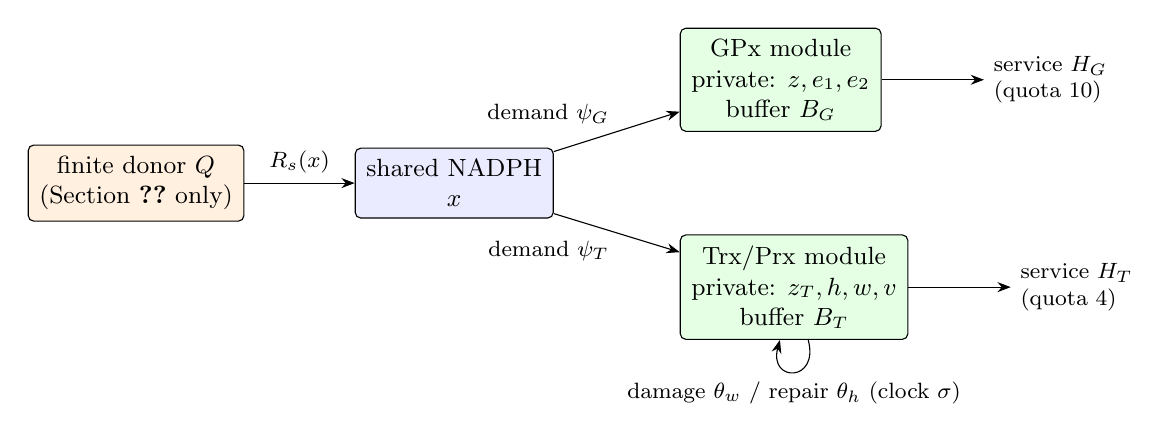
\begin{tikzpicture}[>=Stealth,node distance=9mm and 14mm,
  box/.style={draw,rounded corners=2pt,align=center,inner sep=4pt,font=\small},
  lab/.style={font=\footnotesize}]
\node[box,fill=orange!12] (Q) {finite donor $Q$\\(Section~\ref{sec:duration} only)};
\node[box,fill=blue!8,right=of Q] (x) {shared NADPH\\$x$};
\node[box,fill=green!10,above right=2mm and 16mm of x] (G) {GPx module\\private: $z,e_1,e_2$\\buffer $B_G$};
\node[box,fill=green!10,below right=2mm and 16mm of x] (T) {Trx/Prx module\\private: $z_T,h,w,v$\\buffer $B_T$};
\node[right=13mm of G,lab,align=left] (HGo) {service $\HG$\\(quota $10$)};
\node[right=13mm of T,lab,align=left] (HTo) {service $\HT$\\(quota $4$)};
\draw[->] (Q) -- node[above,lab]{$R_s(x)$} (x);
\draw[->] (x) -- node[above left=-1pt,lab]{demand $\psi_G$} (G);
\draw[->] (x) -- node[below left=-1pt,lab]{demand $\psi_T$} (T);
\draw[->] (G) -- (HGo);
\draw[->] (T) -- (HTo);
\path[->] (T) edge[loop below,looseness=4] node[below,lab]{damage $\theta_w$ / repair $\theta_h$ (clock $\sigma$)} (T);
\end{tikzpicture}
\caption{Accounts in the shared-NADPH model. Service $H_i$ and resource demand
$\psi_i$ differ whenever a module's buffer $B_i$ changes. Arrows summarize
currents of the declared ODE, not elementary stoichiometry. Peroxide and the
repair donor are maintained; the regeneration donor is finite only in
Section~\ref{sec:duration}.}
\label{fig:accounts}
\end{figure}

\subsection{Service, demand, and storage}
The service currents $\HG,\HT$ are not the instantaneous NADPH demands
$\psi_G,\psi_T$. Let
\begin{equation}\label{eq:storage}
B_G=z-1.78+e_1+e_2,\qquad B_T=z_T-.075,\qquad W=234.43+x-B_G-B_T.
\end{equation}
Direct differentiation of \eqref{eq:ode} gives, for every $s$ and $\sigma$,
\begin{equation}\label{eq:account}
\dot B_G=\HG-\psi_G,\qquad \dot B_T=\HT-\psi_T,\qquad \dot W=R_s-\HG-\HT.
\end{equation}
On the physical region $B_G\le234$ (from $2z+e_2\le371.56$ and
$e_1+e_2\le50$) and $B_T\le.43$, so $W\ge0$. The constant $234.43$ only
normalizes $W$ to be nonnegative; differences of $W$, not its origin, enter
every bound. The account \eqref{eq:account} is for regeneration against
service. It must not be merged with peroxide removal: since
$\dot r=\HT-\theta_r$,
\begin{equation}\label{eq:peroxide}
\HG+\theta_r+\theta_w=\HG+\HT+\theta_h+\dot w-\dot r,
\end{equation}
so peroxide consumption, service, and repair differ in transients.

The storage identity is not specific to this chemistry.

\begin{proposition}[Storage account]\label{prop:storage}
Let modules $i=1,\dots,m$ have buffers with $\dot B_i=H_i-D_i$, let the shared
resource satisfy $\dot x=J-\sum_iD_i$, and let a donor satisfy $\dot Q=-J$,
all in common stoichiometric equivalents. Put $W=x-\sum_iB_i+C$ for a constant
$C$. Then
\begin{equation}\label{eq:total}
(Q+W)'=-\sum_iH_i .
\end{equation}
If $W\ge0$ and $Q\ge0$ along a solution on $[a,b]$, then
$\int_a^b\sum_iH_i\dd t\le Q(a)+W(a)$. In particular, total service
$\sum_iH_i\ge q>0$ on $[a,b]$ forces
\[
b-a\le\frac{Q(a)+W(a)}{q},
\]
and no solution with finite initial donor, no replenishment, $Q\ge0$ and
$W\ge0$ has $\sum_iH_i\ge q>0$ for all large times. \evid{conventional}
\end{proposition}
\begin{proof}
Add the three balance laws to get \eqref{eq:total}; integrate and use
$Q(b)+W(b)\ge0$.
\end{proof}
The proposition is a conservation statement under its stated units. It is not
a thermodynamic theorem, and it gives no useful lower bound on the stock needed
for a short mission, because $W(a)$ may be large. That question is settled by
trajectories in Section~\ref{sec:duration}.

\section{Capacity, and what it cannot determine}\label{sec:capacity}

\subsection{The inherited stationary criterion}
Eliminating private states at stationarity gives each branch a strictly
increasing service current $j_i(x)$, so that a quota $j_i\ge q_i$ is an NADPH
floor $x\ge X_i$. Write $J=j_G+j_T$ and $L=\max_iX_i$.

\begin{theorem}[\citep{companionNADPH}]\label{thm:capacity}
For $\sigma=1$ and quotas $(10,4)$, a physical stationary state of
$F_{s,1}$ meeting both quotas exists if and only if
\begin{equation}\label{eq:smin}
s\ge s_{\min}=\frac{J(L)}{R_1(L)},\qquad
L=X_T=\frac{460180}{489387},\qquad .11371266\le s_{\min}\le.11371268 .
\end{equation}
For each $s$ the full stationary state is unique. The numerator is kinetic
demand $J(L)\approx14.3489$, which exceeds the quota sum $14$ by the kinetic
overdelivery of the GPx branch. \evid{inherited; Lean in the companion paper}
\end{theorem}

The nominal source $s=.12$ exceeds $s_{\min}$ by $5.5\%$, and the setting
$s=.1$ fails. We use \eqref{eq:smin} only as the stationary benchmark.
A redesign of an enzyme inventory, as in \citep{companionNADPH}, changes the
transient field, so it does not inherit the dynamic certificates below without
a new check.

\subsection{A matched family with the same stationary states}

\begin{proposition}[Matched repair rates]\label{prop:stationary}
For every $s$ and every $\sigma>0$, the stationary states of $F_{s,\sigma}$
are exactly those of $F_{s,1}$. Hence every stationary service curve, quota
floor, and threshold, in particular Theorem~\ref{thm:capacity}, is the same for
all $\sigma>0$. \evid{Lean}
\end{proposition}
\begin{proof}
At stationarity the $w$ equation reads $\sigma(.00072h-.003w)=0$, which is
equivalent to its $\sigma=1$ version. When it holds, the two exchange terms
cancel in the $h$ equation. The other six equations do not contain $\sigma$.
Both implications hold.
\end{proof}
This is equality of stationary equations. It is not a time reparametrization
of the transient system, because only the two exchange currents $\theta_w,\theta_h$ are rescaled.

\subsection{The hidden clock}

\begin{proposition}[Hidden clock, general form]\label{prop:clockgen}
Let $w:[0,t_1]\to[0,\infty)$ be $C^1$ with $\dot w\ge-\kappa\sigma w$ for
constants $\kappa,\sigma>0$, and suppose a service condition implies
$w\le w_q$ for some $0<w_q<w(0)$. Then every time $t$ at which the service
condition holds satisfies
\begin{equation}\label{eq:clockgen}
t\ge\frac{1}{\kappa\sigma}\log\frac{w(0)}{w_q}.
\end{equation}
Consequently, if a set of descriptors is the same for all $\sigma>0$, no
finite deadline that is a function of those descriptors and of $w(0)$ alone is
valid for all $\sigma>0$. \evid{conventional}
\end{proposition}
\begin{proof}
$(e^{\kappa\sigma t}w)'\ge0$, so $w(t)\ge w(0)e^{-\kappa\sigma t}$; service at
time $t$ needs $w(0)e^{-\kappa\sigma t}\le w_q$. The right side of
\eqref{eq:clockgen} is unbounded as $\sigma\to0$.
\end{proof}

\begin{proposition}[Repair clock in the model]\label{prop:clock}
Let $u$ be a physical solution of \eqref{eq:ode} with any source law and
$\sigma>0$. Put $w_q=19.096-4/(2.1\cdot.43)\approx14.666$. If $w(0)>w_q$,
every $t$ with $\HT(u(t))\ge4$ satisfies
\begin{equation}\label{eq:clock}
t\ge\frac{\log\bigl(w(0)/w_q\bigr)}{.003\,\sigma}.
\end{equation}
\evid{conventional; the inequality $\dot w\ge-.003\sigma w$ and its
integrating-factor form are Lean lemmas}
\end{proposition}
\begin{proof}
Since $h\ge0$, $\dot w=\sigma(.00072h-.003w)\ge-.003\sigma w$. Physicality
gives $y\le.43$ and $v\le19.096-w$, so $\HT\le2.1(.43)(19.096-w)$ and
$\HT\ge4$ implies $w\le w_q$. Apply Proposition~\ref{prop:clockgen}.
\end{proof}

For the physical preparation with $w(0)=.95\cdot19.096$ the bound is
$70.877/\sigma$ seconds. It holds at every regeneration strength. It is an
$\Omega(1/\sigma)$ \emph{necessary} delay: it is not an upper bound, not a sharp
asymptotic, and it does not prove eventual recovery. Numerical quota crossings
for this preparation are later still, near $537$~s at $\sigma=1$
(Figure~\ref{fig:clock}). What the two propositions establish together is an
exact non-identifiability: stationary states, stationary service curves and
pool totals do not determine the repair clock, so they determine no deadline.
A modeler needs a bound on initial retained damage and the repair kinetics.
Whether those can be estimated from a given assay is a separate, practical
identifiability question; a derivative-based estimate of $\sigma$ is
ill-conditioned near repair balance.

\begin{figure}[t]\centering

\includegraphics[width=.95\linewidth]{repair_clock.pdf}
\caption{Stationary information loses the repair clock. Left: the eliminated
stationary service responses, with quotas dotted, are identical for all
$\sigma>0$. Right: the necessary delay \eqref{eq:clock} for the $95\%$
hyperoxidized preparation, and numerical crossing times, which are
observations and not certified deadlines.}
\label{fig:clock}
\end{figure}

\section{A constructive operating certificate}\label{sec:certificate}

\subsection{A moving-box lemma}
The positive results rest on one elementary lemma about time-dependent boxes.
It is a finite simultaneous-face version of Nagumo's tangency condition
\citep{nagumo1942,blanchini1999}, stated so that corners, boundary initial
states and piecewise-affine motion need no separate treatment.

\begin{lemma}[Moving box]\label{lem:box}
Let $a:[t_0,t_1]\to\R^n$ be a $C^1$ solution of $\dot a=f(t,a)$ and let
$q:[t_0,t_1]\to[0,\infty)^n$ be $C^1$. Suppose that for every
$t\in[t_0,t_1]$, every index $i$, every sign $\eta\in\{-1,1\}$, and every
$a$ with $|a_j|\le q_j(t)$ for all $j$ and $a_i=\eta q_i(t)$,
\begin{equation}\label{eq:facecond}
\eta f_i(t,a)<\dot q_i(t).
\end{equation}
If $|a_j(t_0)|\le q_j(t_0)$ for all $j$, then $|a_j(t)|\le q_j(t)$ for all
$j$ and all $t\in[t_0,t_1]$. \evid{conventional; the fixed-rate version used
for Theorem~\ref{thm:main} is a Lean lemma}
\end{lemma}
\begin{proof}
Let $t^*$ be the supremum of times up to which all $2n$ inequalities hold. By
continuity they hold at $t^*$. Suppose $t^*<t_1$. For a face that is active at
$t^*$, the function $g=q_i-\eta a_i$ has $g(t^*)=0$ and, by
\eqref{eq:facecond} applied at the point $a(t^*)$, $\dot g(t^*)>0$; so $g>0$ on
an interval to the right of $t^*$. For an inactive face $g(t^*)>0$ and
continuity gives the same. There are finitely many faces, so all inequalities
hold slightly beyond $t^*$, a contradiction.
\end{proof}
The lemma is applied on consecutive time intervals and joined at the
endpoints, where only the inclusion is needed. With a moving center $c(t)$
one applies it to $a=M^{-1}(u-c(t))$, whose field contains the drift term
$-M^{-1}\dot c(t)$; omitting that term would invalidate the argument.

\subsection{Geometry and the nominal theorem}
The certificate fixes an invertible rational matrix $M$, its exact inverse,
and a rational center
\begin{equation}\label{eq:center}
c\simeq(1.661997,\,3.726108,\,.710658,\,.00284263,\,.211599,\,.302703,\,.0726486,\,7.369302).
\end{equation}
$M=\widehat Q\,\mathrm{diag}(\rho)$, where $\widehat Q$ is a ten-digit rational
rounding of an eigenvector matrix of $DF_{3/25,1}$ near its equilibrium and
$\rho$ is a vector of scales. $M$ approximately separates linear modes, with
rates from about $3641~\mathrm s^{-1}$ (the intermediate $e_2$) to
$.003~\mathrm s^{-1}$ (repair); it is not an exact diagonalization, $c$ is not
assumed stationary, and every residual coupling is bounded in the proof. The
exact data are in the supplementary file \path{data/modal_box.json}
(Appendix~\ref{sec:repro}). For $q\in\R^8_{\ge0}$ put
$\mathcal B(q)=\{c+Ma:|a_i|\le q_i\}$ and
\begin{align}
R&=(.9,.834,.7,.7,.7,.7,.7,.7),& S&=(.9,.7,.7,.7,.7,.7,.7,.7),\nonumber\\
\RR&=\mathcal B(R),\quad\SSS=\mathcal B(S),& \tau&=1/250.\label{eq:radii}
\end{align}
These are correlated parallelepipeds. A state $u_0$ lies in $\RR$ if and only
if $|M^{-1}(u_0-c)|\le R$ componentwise. A reference deficient preparation is
\begin{equation}\label{eq:prep}
\begin{aligned}
p=c+\tfrac56M_{\cdot1}\simeq(&1.692492,\,3.730262,\,.710652,\,.00284261,\\
&.249285,\,.302574,\,.0726486,\,7.357791),
\end{aligned}
\end{equation}
which has $\HT(p)\approx3.951<4$, and
$\Pp=\{u:|u_j-p_j|\le5\cdot10^{-7}\}$ is an independent box around it.

\begin{theorem}[Nominal operational service]\label{thm:main}
Every state in $\Pp$ is physical, lies in $\RR$, and has $\HT<4$. For every
$u_0\in\RR$, the system \eqref{eq:ode} with $(s,\sigma)=(3/25,1)$ has a unique
forward solution $u$ with $u(0)=u_0$. It is physical and lies in $\RR$ for all
$t\ge0$, and lies in $\SSS$ for all $t\ge\tau$. On this solution
\begin{equation}\label{eq:floors}
\HG\ge\tfrac{207}{20}\ (t\ge0),\qquad \HT\ge\tfrac{391}{100}\ (t\ge0),\qquad
\HT\ge\tfrac{401}{100}\ (t\ge\tau).
\end{equation}
For every $T\ge0$,
\begin{equation}\label{eq:deficit}
\int_0^T\pos{10-\HG}\dd t=0,\qquad \int_0^T\pos{4-\HT}\dd t\le\frac{9}{25000},
\end{equation}
and for every $a\ge\tau$ and $T\ge0$,
\begin{equation}\label{eq:windows}
\int_a^{a+T}\!\HG\dd t\ge10.35\,T,\quad
\int_a^{a+T}\!\HT\dd t\ge4.01\,T,\quad
\int_a^{a+T}\!R_{3/25}(x)\dd t\ge14.36\,T-.1 .
\end{equation}
Thus Definition~\ref{def:spec} holds with $\Pp_0=\RR$, $\tau=4$~ms,
$H=\infty$, $d_G=0$ and $d_T=3.6\cdot10^{-4}~\uM$. \evid{Lean}
\end{theorem}

Existence, physicality, capture and uniqueness are conclusions. The theorem
does not assume an attracting equilibrium or that a proposed trajectory stays
physical. An earlier certificate for the same field had deadline $2000$~s,
because it shrank every modal coordinate at a common slow rate. The factor
$5\cdot10^{5}$ between the two deadlines measures certificate conservatism,
not chemistry: service recovery needs only the second-fastest mode to relax,
while the slow repair coordinate may stay where it is.

\subsection{Proof of Theorem~\ref{thm:main}}\label{sec:proof}
\paragraph{Field expansion.}
Write $a=M^{-1}(u-c)$ and $f(a)=M^{-1}F_{3/25,1}(c+Ma)$, and let
$A=M^{-1}DF_{3/25,1}(c)M$ and $b=M^{-1}F_{3/25,1}(c)$. Then
\begin{equation}\label{eq:modal}
f(a)=b+Aa+N(a),\qquad |N_i(a)|\le n_i\quad(|a_j|\le1),
\end{equation}
with rational $n_i$ obtained as follows. Put $d=Ma$ and $w_j=\sum_k|M_{jk}|$.
The polynomial part of $F$ is quadratic, and its second-order remainder is a
fixed linear combination of five products,
\[
d_0d_1,\quad d_0d_4,\quad(-2d_1-d_3)d_2,\quad(-2d_1-d_3)d_3,\quad d_4d_7,
\]
bounded by $w_0w_1$, $w_0w_4$, $(2w_1+w_3)w_2$, $(2w_1+w_3)w_3$, $w_4w_7$.
The source remainder is exactly
\begin{equation}\label{eq:source-rem}
-\frac{45\,(57.3)\,d_0^2}{(87.3-c_0)^2(87.3-c_0-d_0)},
\end{equation}
bounded using $87.3-c_0-w_0>0$. The reaction vectors are transformed by
$M^{-1}$ \emph{before} absolute values are taken; this keeps cancellations
that a coordinatewise comparison of the raw field loses, and is why the modal
certificate succeeds where absolute comparisons in physical coordinates fail.
The same enclosures show that the whole unit cube $\mathcal B(\mathbf 1)$ is
strictly physical, with $1.60<x<1.73$.

\paragraph{Face budgets.}
For $q\le\mathbf1$ define
\begin{equation}\label{eq:budget}
D_i(q)=A_{ii}q_i+\sum_{j\ne i}|A_{ij}|q_j+|b_i|+n_i .
\end{equation}
On a face $a_i=\eta q_i$ with $|a_j|\le q_j$, \eqref{eq:modal} gives
$\eta f_i(a)\le D_i(q)$. Let $v=(0,-67/2,0,\dots,0)$. Exact evaluation
(Table~\ref{tab:faces}) gives
\begin{equation}\label{eq:face-checks}
D_i(R)<v_i,\qquad D_i(S)<v_i\qquad(0\le i<8).
\end{equation}

\begin{table}[t]\centering\small
\caption{Signed face budgets (rounded; the strict inequalities use exact
rationals). Only modal coordinate $1$ has a moving face.}
\label{tab:faces}
\begin{tabular}{rrrr@{\qquad}rrrr}\toprule
$i$&$D_i(R)$&$D_i(S)$&$v_i$&$i$&$D_i(R)$&$D_i(S)$&$v_i$\\\midrule
0&$-3274.3640$&$-3274.3652$&0&4&$-.33539200$&$-.33539200$&0\\
1&$-41.1928$&$-34.3435$&$-33.5$&5&$-.11454379$&$-.11454379$&0\\
2&$-.66394145$&$-.66394147$&0&6&$-.02972857$&$-.02972857$&0\\
3&$-.77105616$&$-.77105622$&0&7&$-.00049735$&$-.00049742$&0\\
\bottomrule\end{tabular}
\end{table}

\paragraph{Capture, existence, physicality.}
On $[0,\tau]$ let $q(t)=(1-250t)R+250tS$, so $\dot q=v$. Since $D_i$ is affine
in $q$, \eqref{eq:face-checks} gives $D_i(q(t))<v_i$, which is
\eqref{eq:facecond}. Lemma~\ref{lem:box} keeps the solution in
$\mathcal B(q(t))$, including from boundary and corner initial states. At
$t=\tau$ the solution is in $\SSS$; since $D_i(S)<v_i\le0$, the lemma with
constant radius makes $\SSS$ forward invariant, and likewise $\RR$. The field
is smooth on $x<87.3$ and the barriers confine any local solution to a compact
subset of that domain, so the solution continues for all time and is unique.
The Lean development realizes the same continuation through a globally
Lipschitz extension of the field that agrees with it on the invariant region.

\paragraph{Outputs, preparation, accounts.}
For a radius $q$ let $d_j(q)=\sum_k|M_{jk}|q_k$. From $|u_j-c_j|\le d_j(q)$,
\begin{equation}\label{eq:outputs}
\HG\ge L_G(q)=.21\bigl(50-c_2-c_3-d_2-d_3\bigr),\qquad
\HT\ge L_T(q)=2.1\bigl(.505-c_4-d_4\bigr)\bigl(c_7-d_7\bigr),
\end{equation}
with $L_G(R),L_G(S)>10.35$, $L_T(R)>3.91$, $L_T(S)>4.01$. For $u\in\Pp$,
$|[M^{-1}(u-c)]_i|\le\frac56\mathbf 1_{i=1}+\varepsilon\sum_j|(M^{-1})_{ij}|\le R_i$
with $\varepsilon=5\cdot10^{-7}$, and
$\HT(u)\le2.1(.505-p_4+\varepsilon)(p_7+\varepsilon)<3.9512$. The floors give
\eqref{eq:deficit}: the Trx shortfall is at most $.09$ for a time $\tau$. With
$\ell=(1,-1,-1,-1,-1,0,0,0)$ one has $W(c+Ma)=W(c)+\ell Ma$, and on $\SSS$
the range of $W$ is
\begin{equation}\label{eq:W-range}
2\sum_i|(\ell M)_i|S_i=\frac{2430664273305669}{25000000000000000}<\frac1{10}.
\end{equation}
Integrating \eqref{eq:account} along the solution,
$\int_a^{a+T}R_{3/25}\dd t=\int_a^{a+T}(\HG+\HT)\dd t+W(u(a+T))-W(u(a))$,
which gives the last bound of \eqref{eq:windows}. The subtracted $.1$ is
storage on $\SSS$; it does not come from summing quotas.\qed

\subsection{Preparation geometry and an independent tolerance}
\label{sec:geometry}
The box $\Pp$ has halfwidth $0.5$~pM, which is a legitimate concern if read as
the tolerance of the theorem. It is not: the theorem covers all of $\RR$,
whose coordinate projections have halfwidths
\[
(48,\ 27,\ .15,\ .0012,\ 39,\ 1.4,\ .11,\ 53)\ \text{nM}
\]
in the order of $u$. The projections are wide but correlated, and their
product is not contained in $\RR$. For an independent box with center $p'$ and
halfwidths $\epsilon_j$, a sufficient membership test is the finite linear
condition
\begin{equation}\label{eq:membership}
|M^{-1}(p'-c)|+|M^{-1}|\,\epsilon\le R .
\end{equation}
Around $p$, the largest uniform halfwidth allowed by \eqref{eq:membership} is
$0.633$~pM. The binding row is modal coordinate $0$, the $3641~\mathrm s^{-1}$
mode of the intermediate $e_2$, whose scale $\rho_0=10^{-6}$ is tiny because
$e_2\approx2.8$~nM is itself tiny. Coordinate by coordinate the test allows
$x\pm0.48$~nM, $z\pm2.0$~nM, $v\pm2.6$~nM, $w\pm0.11$~nM, but only
$e_2\pm0.64$~pM. The narrow box is therefore a property of the chosen modal
scales in rapidly equilibrating directions, not of the chemistry, and it can be
removed without changing the Lean theorem: fast directions may start far
outside $\RR$ and still arrive in $\SSS$ quickly.

\begin{corollary}[Independent $0.1\%$ preparations]\label{cor:box}
Let $\Pp_\kappa=\{u:|u_j-p_j|\le\kappa p_j,\ 0\le j<8\}$ with
$\kappa=10^{-3}$. Then $\Pp\subset\Pp_\kappa$, every state of $\Pp_\kappa$ is
physical and has $\HT<4$, and for every $u_0\in\Pp_\kappa$ the nominal system
has a unique global physical solution with
\[
\HG\ge10\ (t\ge0),\qquad \HT\ge4\ (t\ge\tau),\qquad
\int_0^\infty\pos{4-\HT}\dd t\le1.1\cdot10^{-4}~\uM,
\]
and $u(t)\in\SSS$ for all $t\ge1/4+\tau$, after which all conclusions of
Theorem~\ref{thm:main} hold. \evid{exact tube on $[0,1.004]$, then Lean}
\end{corollary}
\begin{proof}
$\Pp_\kappa\subset p+M\mathcal B_0(q_0)$, where
$\mathcal B_0(q)=\{a:|a_j|\le q_j\}$ and
\[
q_{0,i}=\kappa\sum_j|(M^{-1})_{ij}|\,p_j,\qquad
q_0\approx(8.06,\ .0101,\ 10.7,\ 27.0,\ 2.39,\ .207,\ .303,\ .483);
\]
coordinates $0,2,3,4$ start far outside $\RR$. The tube certificate of Appendix~\ref{sec:tube} with the
maintained source verifies the hypotheses of Lemma~\ref{lem:box} on $1206$
steps covering $[0,1.004]$, with service floors $\HG\ge10.3499$ throughout and
$\HT\ge4$ from $2.75$~ms, and $\HT\ge4.034$ on $[\tau,1.004]$. The slice at the
grid time $t^*=6191921/25000000<1/4$ satisfies
$|M^{-1}(\bar c(t^*)-c)|+q(t^*)\le S$ componentwise,
so $u(t^*)\in\SSS\subset\RR$. Theorem~\ref{thm:main} then applies from $t^*$:
$u(t)\in\SSS$ for $t\ge t^*+\tau$, while the tube covers $[0,t^*+\tau]$.
The shortfall bound is the exact sum $\sum_k h_k\pos{4-L_{T,k}}$ over steps
before $\tau$.
\end{proof}
The independent tolerances are now $x\pm1.7$~nM, $z\pm3.7$~nM,
$e_1\pm0.71$~nM, $e_2\pm2.8$~pM, $z_T\pm0.25$~nM, $h\pm0.30$~nM,
$w\pm73$~pM and $v\pm7.4$~nM, simultaneously. The binding quantity is no longer
geometry but the service margin: a $0.2\%$ box still passes the mission checks
in floating point but leaves $\HT-4<.011$ at $\tau$ and does not enter $\SSS$
by one second, so we do not claim it. These are deterministic neighborhoods.
They are not stochastic confidence statements; intrinsic-noise claims would
need a compartment volume and a stochastic model
\citep[cf.][]{companionReliable}.

\begin{figure}[t]\centering

\includegraphics[width=.95\linewidth]{recovery.pdf}
\caption{Recovery under the maintained source $s=.12$. The band is the
exact-arithmetic enclosure of $\HT$ over all preparations in the $0.1\%$ box
$\Pp_\kappa$ (Corollary~\ref{cor:box}); the solid curve is a numerical solution
from $p$. Dashed: the Lean-checked floors of Theorem~\ref{thm:main}, valid on
all of $\RR$. The numerical curve crosses the quota near $1.68$~ms; the curve
is an illustration, the band and floors are proofs.}
\label{fig:recovery}
\end{figure}

\subsection{Continuous source uncertainty}
\begin{theorem}\label{thm:robust}
Let $s:[0,\infty)\to\R$ be continuous with $|s(t)-3/25|\le\delta=10^{-6}$. For
every $u_0\in\RR$ the system $\dot u=F_{s(t),1}(u)$ has a unique global forward
solution, and all conclusions of Theorem~\ref{thm:main} hold, with the
expenditure bound stated for the actual current $R_{s(t)}(x(t))$.
\evid{conventional; inequality \eqref{eq:robust-checks} Lean}
\end{theorem}
\begin{proof}
$M^{-1}\bigl(F_{s,1}(u)-F_{3/25,1}(u)\bigr)=M^{-1}e_x\,(s-3/25)R_1(x)$ and
$0\le R_1\le130$ on the physical region, so the modal perturbation in
coordinate $i$ is at most $E_i=130\,\delta\,|(M^{-1})_{i0}|$. Exact checks give
\begin{equation}\label{eq:robust-checks}
D_i(R)+E_i<v_i,\qquad D_i(S)+E_i<v_i .
\end{equation}
The perturbed face condition \eqref{eq:facecond} follows by affine
interpolation, pointwise in $s$ and with no derivative of $s$. The field is
continuous in $t$ and locally Lipschitz in $u$, so Picard--Lindel\"of,
Lemma~\ref{lem:box} and compact continuation \citep{walter1998} give the
solution. Output bounds depend only on the rectangles, and \eqref{eq:account}
holds with the actual source.
\end{proof}
The band is a sufficient certificate, not an uncertainty model or a robustness
threshold; discontinuous switching is outside the statement.

\section{Costs and finite duration}\label{sec:duration}

Append a donor stock $Q$, in donor equivalents per reaction volume, consumed
one equivalent per NADPH regenerated. Peroxide and the repair donor remain
maintained. By Proposition~\ref{prop:storage}, for any such law
\begin{equation}\label{eq:total-stock}
(Q+W)'=-\HG-\HT,
\end{equation}
so no finite stock supports the quotas forever. What a finite stock can do
depends on how the source responds to depletion.

\subsection{Linear donor law: a fixed-band argument}
For a concentration scale $V>0$ let
\begin{equation}\label{eq:donor}
\dot u=F_{Q/V,1}(u),\qquad\dot Q=-R_{Q/V}(x),\qquad Q(0)=Q_0=\tfrac3{25}V .
\end{equation}
$V$ converts stock to the source scale; it is not a geometric volume.

\begin{theorem}[Finite mission, fixed band]\label{thm:donor}
Let $H\ge\tau$ and $V\ge16{,}000{,}000\,H$. For each $u_0\in\RR$,
\eqref{eq:donor} has a unique solution on $[0,H]$; its $u$ component is
physical, stays in $\RR$, lies in $\SSS$ on $[\tau,H]$, and satisfies the
floors and shortfall bounds of Theorem~\ref{thm:main}. Moreover
\begin{equation}\label{eq:donor-tube}
Q_0-16t\le Q(t)\le Q_0,\qquad
14.36\,T-.1\le Q(a)-Q(a+T)\le16\,T\quad(\tau\le a\le a+T\le H).
\end{equation}
\evid{conventional nine-state proof; margins \eqref{eq:robust-checks} Lean}
\end{theorem}
\begin{proof}
The nine-state field is smooth for $x<87.3$. Take the sixteen modal faces
together with $Q\le Q_0$ and $Q\ge Q_0-16t$. On this prospective tube
$|Q/V-3/25|\le16H/V\le\delta$ and $Q\ge(3/25-\delta)V>0$, so
\eqref{eq:robust-checks} applies on the tube without assuming that the
solution stays in it. On the upper donor face $(Q_0-Q)'=R>0$ because $x<30$.
On the lower one $(Q-Q_0+16t)'=16-R_{Q/V}(x)>0$, since $(30-x)/(87.3-x)$ is
decreasing and
$R_{Q/V}(x)\le(3/25+\delta)\,375\cdot30/87.3=120001/7760<16$.
Lemma~\ref{lem:box}, applied to all eighteen faces, and compact continuation
give the solution. The bounds \eqref{eq:donor-tube} follow from
\eqref{eq:total-stock}, the floors, and \eqref{eq:W-range}.
\end{proof}

For the one-second service window $[.004,1.004]$ this needs
$V=16{,}064{,}000$, that is $Q_0=1{,}927{,}680~\uM\approx1.9$~M, to spend at
most $16.1~\uM$. The reason is structural. The proof keeps the source inside
the band of Theorem~\ref{thm:robust}, and under the linear law that allows
spending only
\begin{equation}\label{eq:ppm}
\frac{Q_0-Q}{Q_0}\le\frac{10^{-6}}{.12}\approx8.3\ \text{parts per million}
\end{equation}
of the stock. Tightening the bound $16$ on the regeneration rate cannot repair
a five-order ratio. Three quantities must be kept apart: equivalents consumed;
inventory the \emph{kinetic law} needs to hold its rate; and reserve added by
the \emph{certificate}. The $1.9$~M figure mixes the last two. We remove the
second by changing the law (Section~\ref{sec:saturating}) and the third by
changing the proof (Section~\ref{sec:tube-result}).

\subsection{A saturating donor law}\label{sec:saturating}
Let the source depend on the donor through a saturating factor with affinity
scale $K>0$, normalized at the initial stock:
\begin{equation}\label{eq:sat}
s_{\mathrm{eff}}(Q)=s_0\,\frac{Q/(K+Q)}{Q_0/(K+Q_0)},\qquad
\dot u=F_{s_{\mathrm{eff}}(Q),1}(u),\qquad\dot Q=-R_{s_{\mathrm{eff}}(Q)}(x),
\end{equation}
with $s_0=3/25$ and $Q(0)=Q_0$. This is a different model from
\eqref{eq:donor}, not a sharper analysis of it. One equivalent is still
consumed per equivalent regenerated, so \eqref{eq:total-stock} holds.

\begin{corollary}[Saturating donor]\label{cor:saturating}
Let $H\ge\tau$, $D=16H$, $\delta=10^{-6}$, and $Q_0>D$ with
\begin{equation}\label{eq:satcond}
\frac{s_0KD}{Q_0\,(K+Q_0-D)}\le\delta,
\quad\text{equivalently}\quad
Q_0\ge\frac{D-K+\sqrt{(D-K)^2+4(s_0/\delta)KD}}{2}.
\end{equation}
Then every conclusion of Theorem~\ref{thm:donor} holds for \eqref{eq:sat} on
$[0,H]$, for every $u_0\in\RR$. \evid{conventional; identity
\eqref{eq:satdrop}, its bound and both examples Lean}
\end{corollary}
\begin{proof}
For $Q_0-D\le Q\le Q_0$,
\begin{equation}\label{eq:satdrop}
0\le s_0-s_{\mathrm{eff}}(Q)=\frac{s_0K(Q_0-Q)}{Q_0(K+Q)}\le\frac{s_0KD}{Q_0(K+Q_0-D)}\le\delta .
\end{equation}
The proof of Theorem~\ref{thm:donor} now applies verbatim on the tube
$Q_0-16t\le Q\le Q_0$: the source stays in the checked band, and
$R\le(3/25)\,375\cdot30/87.3<16$ on the lower donor face. Equality in
\eqref{eq:satcond} is allowed because the face inequalities
\eqref{eq:robust-checks} are strict. The quadratic form follows by clearing
denominators in \eqref{eq:satcond}, whose positive root exceeds $D$.
\end{proof}

For $H=251/250$ (so $D=16.064~\uM$), two exact instances are
\begin{align*}
(Q_0,K)=(200~\uM,\ .01~\uM):&\qquad s_0-s_{\mathrm{eff}}\le\tfrac{753}{1437078125}\approx5.24\cdot10^{-7},\\
(Q_0,K)=(1500~\uM,\ 1~\uM):&\qquad s_0-s_{\mathrm{eff}}\le\tfrac{502}{580053125}\approx8.65\cdot10^{-7}.
\end{align*}
These stocks are $9638$ and $1285$ times smaller than under the linear law, for
all $u_0\in\RR$ and with the refined floors $10.35$ and $4.01$. When the square
root dominates, \eqref{eq:satcond} scales like $\sqrt{s_0KD/\delta}$; the exact
formula, not this approximation, should be used for long horizons. The values
of $K$ are not fitted or attributed to a donor--enzyme pair; an experimental
realization would need capacity, affinity and stock to be separately
identifiable. The corollary also shows how a dynamic compatibility theorem is
reused: a new supply is admissible when its \emph{coupled} depletion keeps it
inside a proved operating envelope, and the envelope must be verified on the
coupled tube.

\subsection{Linear donor law: the depleted trajectory}\label{sec:tube-result}
We return to the unchanged law \eqref{eq:donor} and certify the trajectory that
actually occurs, letting the source fall far outside the band.

\begin{theorem}[Buffered finite mission]\label{thm:tube}
Let $H=1.004$, let $u_0\in\Pp_\kappa$ with $\kappa=10^{-3}$ as in
Corollary~\ref{cor:box} (so $\HT(u_0)<4$), and let
$|Q(0)-\tfrac3{25}V|\le10^{-3}~\uM$ in \eqref{eq:donor}.
\begin{enumerate}[label=(\alph*)]
\item \emph{$V=1000$, $Q_0=120~\uM$: success.} There is a unique solution on
$[0,H]$; it is physical, and
\[
\HG\ge10.3499\ \ (0\le t\le H),\quad \HT\ge4.034\ \ (\tau\le t\le H),\quad
\int_0^H\!\pos{4-\HT}\dd t\le1.1\cdot10^{-4} .
\]
The donor spent on $[\tau,H]$ lies in $[14.034,14.045]~\uM$ and the final
source scale in $[.10589,.10591]$. For all $t\ge.434$ one has
$s(t)=Q(t)/V<.1137126\le s_{\min}$. The storage drawdown satisfies
\begin{equation}\label{eq:drawdown}
\int_0^H(\HG+\HT)\dd t-\int_0^HR_{Q/V}(x)\dd t=W(u(0))-W(u(H))\in[.700,.751]~\uM .
\end{equation}
\item \emph{$V=500$, $Q_0=60~\uM$: failure.} There is a unique physical
solution on $[0,H]$, and $\HT(u(H))\le3.9132<4$. The mission of
Definition~\ref{def:spec} with $\tau=.004$ and $H=1.004$ fails from every
preparation in $\Pp_\kappa$.
\end{enumerate}
\evid{exact rational tube certificates, replayable; not kernel-checked}
\end{theorem}
The proof is the certificate of Appendix~\ref{sec:tube}: a piecewise-affine
reference $(\bar c(t),\bar C(t))$ for the state and the spent donor, affine
radii, and $9$ strict face inequalities on each of $1206$ time steps, which
verify the hypotheses of Lemma~\ref{lem:box} for the nine-state system
uniformly in time. Every inequality is evaluated in exact rational arithmetic.

Three points deserve emphasis. First, the certified sufficient stock falls
from $1.9$~M to $120~\uM$ under the \emph{same} law, a factor $16{,}064$, and
the sufficient and insufficient stocks differ by a factor of two. A numerical
bisection from $p$ places the threshold near $70.9~\uM$, and a numerical
solution with $Q_0=120~\uM$ holds the Trx quota until about $1.387$~s; these
two numbers are observations. Second, the success in (a) is not a refinement of
the stationary picture but runs against it: for the last $57\%$ of the mission
the source is below $s_{\min}$, where by Theorem~\ref{thm:capacity} \emph{no}
stationary state meets both quotas, and yet both quotas are met with margin.
By \eqref{eq:drawdown}, about $0.7~\uM$ of the $14.8~\uM$ of delivered service
is paid from stored reduced carrier rather than from regeneration. A rule that
applies the stationary threshold at each instant would reject a mission that
provably succeeds. Third, the old storage range \eqref{eq:W-range} is not used:
it belongs to $\SSS$, which the depleted trajectory leaves, and the accounts in
(a) are computed on the actual tube.

We could not extend (a) to all of $\RR$, and the obstruction is physical rather
than technical: $\RR$ contains states whose nominal floor is only
$\HT\ge4.01$, carried by slow coordinates that do not relax within a second,
and a $12\%$ fall of the source removes that margin.

\begin{figure}[t]\centering

\includegraphics[width=\linewidth]{donor.pdf}
\caption{Finite donor. Left: certified sufficient stock for the one-second
mission: the saturating-law curve \eqref{eq:satcond} against affinity scale,
and the two linear-law results as horizontal lines; curves for different laws
are not one ``optimal stock'' curve. Middle: $\HT$ for the linear law with
$Q_0=120$ and $60~\uM$; bands are exact enclosures over $\Pp_\kappa$ and donor
tolerance, curves are the certificate references. Right: the source scale
falls below the stationary threshold $s_{\min}$ at $t\approx.43$~s for
$Q_0=120~\uM$ while the quota continues to hold.}
\label{fig:donor}
\end{figure}

\section{A worked comparison}\label{sec:worked}
Table~\ref{tab:worked} places the three questions side by side, for one
chemistry, one pair of quotas and common units.

\begin{table}[!ht]\centering\small
\caption{What limited information predicts and what the full-state analysis
shows. All rows use quotas $(10,4)$~\fluxunit.}
\label{tab:worked}
\begin{tabular}{>{\raggedright\arraybackslash}p{.25\linewidth}>{\raggedright\arraybackslash}p{.27\linewidth}>{\raggedright\arraybackslash}p{.38\linewidth}}
\toprule
Situation & From stationary data & Full-state conclusion\\\midrule
Adequate source $s=.12$; small oxidation defect ($\Pp_\kappa$, $\HT(u_0)<4$)
& Compatible ($s>s_{\min}$); no deadline
& Both quotas from $4$~ms on, forever; Trx shortfall $\le1.1\cdot10^{-4}~\uM$; regeneration $\ge14.36T-.1$ on later windows (Thm.~\ref{thm:main}, Cor.~\ref{cor:box})\\
Same stationary responses; $95\%$ hyperoxidized pool; repair scale $\sigma$
& Compatible, identically for all $\sigma$
& No service before $70.9/\sigma$~s at any source strength (Prop.~\ref{prop:clock}); observed $\approx537$~s at $\sigma=1$\\
Linear donor, $Q_0=120~\uM$, one-second mission
& Incompatible for $t\ge.43$~s ($s<s_{\min}$)
& Mission succeeds with $\HT\ge4.034$; $0.70$--$0.75~\uM$ drawn from storage (Thm.~\ref{thm:tube}a)\\
Linear donor, $Q_0=60~\uM$
& Incompatible for $t\ge.22$~s
& Mission fails: $\HT(u(H))\le3.913$ (Thm.~\ref{thm:tube}b)\\
Any finite donor, indefinite service
& not addressed
& Impossible (Prop.~\ref{prop:storage})\\
\bottomrule
\end{tabular}
\end{table}

The first two rows have the same stationary description and recovery times
that differ by more than four orders of magnitude; the difference is retained
private state. The third row is a case where the stationary threshold is
pessimistic. In an assay, $x$ corresponds to measured NADPH, service to branch
peroxide-reduction flux, and $w$ to the sulfinylated peroxiredoxin fraction;
the quotas are design values and are not thresholds of cellular health.

\section{Discussion and limits}\label{sec:discussion}

\paragraph{What a modeler needs.}
To guarantee joint service one needs more than branch response curves. For
\emph{capacity}, the curves and the source suffice \citep{companionNADPH}. For
\emph{recovery}, one needs a bound on the initial private state in the
directions that do not relax before the deadline, and the kinetics of the
slowest process that gates service; Proposition~\ref{prop:clockgen} shows this
is unavoidable. For \emph{duration}, one needs the supply law and the stored
account $W$, and the verdict must be read from the depleted trajectory: a
budget computed on an undepleted nominal run is a necessary condition only.

\paragraph{Compositional use.}
For modules $\dot z_i=f_i(x,z_i)$ with outputs $H_i$, demands $D_i$ and
$\dot x=J-\sum_iD_i$, Lemma~\ref{lem:box} can be applied blockwise: bound the
private faces uniformly over a resource interval, and bound the \emph{loaded}
resource faces using those same private sets, all in one first-exit argument.
Assuming a favorable resource trace and then presenting it as a conclusion
about the coupled system would be circular. In the present model interval
bounds on the private blocks destroy signed cancellations between the $x$,
$z_T$ and $v$ directions, which is why the certificates above use joint modal
coordinates.

\paragraph{Limits.}
The positive theorems are sufficient certificates on explicit regions. They
prove no global basin, no optimal deadline, no minimal stock for the linear
law (only the bracket $60$--$120~\uM$), and nothing about the source-$.1$
equilibrium or heavily hyperoxidized preparations beyond the necessary delay.
The $0.1\%$ box is small in absolute terms. The donor models make only
regeneration finite; peroxide and the repair donor remain maintained, so the
model is not thermodynamically closed. Parameters are declared, not
calibrated. The full evolution statements of Theorems~\ref{thm:robust}
and~\ref{thm:donor} and Corollary~\ref{cor:saturating} are conventional proofs
resting on kernel-checked inequalities, and Theorem~\ref{thm:tube} and the
finite-horizon part of Corollary~\ref{cor:box} rest on exact arithmetic that is
replayable but not kernel-checked; a reusable formal nonautonomous comparison
lemma would close the first gap.

\appendix
\section{The moving-tube certificate}\label{sec:tube}

\paragraph{Data.}
A certificate is a list of rational times $0=t_0<\dots<t_n=H$ containing
$\tau$, rational reference points $\bar c_k\in\R^8$ and $\bar C_k\in\R$ for the
state and the spent donor $C=Q_0-Q$, and rational radii $q_k\in\R^8_{>0}$,
$q^C_k>0$. References and radii are affine between grid times. The tube is
\[
u(t)\in\bar c(t)+M\,\mathcal B_0(q(t)),\qquad |C(t)-\bar C(t)|\le q^C(t),
\]
with $\mathcal B_0(q)=\{a:|a_j|\le q_j\}$ and the \emph{same} $M$ as in
Section~\ref{sec:certificate}. The source is $s=\tfrac3{25}-C/V$, with
$1/V=0$ for the maintained source. Reference points are a numerical solution
rounded to $13$ decimals; they carry no evidential weight, because their
residual is bounded exactly. Initial data are $\bar c_0=p$,
$q_{0,i}\ge\kappa\sum_j|(M^{-1})_{ij}|p_j$, $\bar C_0=0$ and $q^C_0=10^{-3}$.

\paragraph{One step.}
Fix a step of length $h$, and let $c_m$, $C_m$ be midpoints, $\Delta$,
$\Delta_C$ the increments, $s_m=\tfrac3{25}-C_m/V$, $J=DF_{s_m,1}(c_m)$,
$A=M^{-1}JM$, $\hat q=\max(q_k,q_{k+1})$ and $\hat q^C$ likewise. In the step,
$u=c_m+d$ with $d=\theta\Delta+Ma$, $|\theta|\le\frac12$, so
$|d_j|\le\hat d_j=\sum_k|M_{jk}|\hat q_k+\frac12|\Delta_j|$, and
$|s-s_m|\le\hat\varsigma=(\hat q^C+\frac12|\Delta_C|)/V$. With
$a=M^{-1}(u-\bar c(t))$,
\[
\dot a=M^{-1}\bigl(F_{s_m,1}(c_m)-\Delta/h\bigr)+\theta M^{-1}J\Delta+Aa
+M^{-1}N(d)+(s-s_m)R_1(x)M^{-1}e_x,
\]
where $N$ is the exact second-order remainder of
Section~\ref{sec:proof} with $c_m,s_m$ in place of $c,\tfrac3{25}$. Hence on
the face $a_i=\eta q_i(t)$,
\begin{equation}\label{eq:stepface}
\begin{aligned}
\eta\dot a_i\le{}& A_{ii}q_i(t)+\sum_{j\ne i}|A_{ij}|\hat q_j
+\bigl|[M^{-1}(F_{s_m,1}(c_m)-\Delta/h)]_i\bigr|\\
&+\tfrac12\bigl|[M^{-1}J\Delta]_i\bigr|
+n_i(\hat d)+\hat\varsigma\,R_1(c_{m,0}-\hat d_0)\,|(M^{-1})_{i0}| ,
\end{aligned}
\end{equation}
using that $R_1$ is positive and decreasing. The first term is affine in $t$
and is replaced by its larger endpoint value. The check is that the right side
is strictly less than $(q_{k+1,i}-q_{k,i})/h$. Radii may grow; slow
coordinates are allowed to, which is what a finite horizon permits and an
invariant set does not. For the donor faces,
\[
\bigl|(C-\bar C)'\bigr|\le\bigl|s_mR_1(c_{m,0})-\Delta_C/h\bigr|
+s_m\frac{375\cdot57.3}{(87.3-c_{m,0}-\hat d_0)^2}\,\hat d_0
+\hat\varsigma\,R_1(c_{m,0}-\hat d_0)<\frac{q^C_{k+1}-q^C_k}{h}.
\]
The thirteen physical margins of \eqref{eq:physical} are checked to be positive
on the whole slice, and the floors \eqref{eq:outputs} are evaluated with
$c_m,\hat d$. Lemma~\ref{lem:box} on each step, joined at grid times, and
compact continuation give existence, uniqueness and the enclosure. Accounts
use endpoint slices: spent donor is $\bar C\pm q^C$, and
$W\in234.43+\ell\bar c\pm\sum_i|(\ell M)_i|q_i$.

\paragraph{Outcome.}
All three certificates use $1206$ steps, geometric from $2\cdot10^{-6}$~s and
then uniform. Table~\ref{tab:tube} lists the verified quantities. The smallest
face margin is positive in each case; it is tiny by design, since radii are
chosen just above what the inequalities need.

\begin{table}[ht]\centering\small
\caption{Verified outcomes of the tube certificates (exact values rounded
outward).}\label{tab:tube}
\begin{tabular}{lrrr}\toprule
&maintained source&$Q_0=120~\uM$&$Q_0=60~\uM$\\\midrule
$\min\HG$ floor on $[\tau,H]$&$10.34995$&$10.34990$&$10.34963$\\
$\min\HT$ floor on $[\tau,H]$&$4.03438$&$4.03438$&$3.87684$\\
$\HT$ enclosure at $H$&$[4.5326,4.5484]$&$[4.2182,4.2421]$&$[3.8770,3.9132]$\\
$\HT\ge4$ certified from (ms)&$2.75$&$2.75$&--\\
Trx shortfall bound (\uM)&$1.017\cdot10^{-4}$&$1.018\cdot10^{-4}$&$1.018\cdot10^{-4}$\\
Regeneration on $[0,H]$ (\uM)&$[14.947,14.953]$&$[14.095,14.104]$&$[13.297,13.310]$\\
Final source scale&$.12$&$[.105896,.105905]$&$[.093381,.093405]$\\
$W(u(0))-W(u(H))$ (\uM)&$[-.035,.013]$&$[.700,.751]$&$[1.374,1.429]$\\
Slice inside $\SSS$ from&$.2477$~s&never&never\\
\bottomrule\end{tabular}
\end{table}

\section{Evidence and reproduction}\label{sec:repro}

\paragraph{Formal evidence.}
The Lean development uses Lean~4 \citep{moura2021}, version 4.30.0, and Mathlib
\citep{mathlib2020} at revision
\begin{center}\small\texttt{c5ea00351c28e24afc9f0f84379aa41082b1188f}.\end{center}
Theorem~\ref{thm:main} is the declaration
\begin{center}\small\texttt{DynamicSharedResource.Certificate.fast\_joint\_service}\end{center}
in \path{proofs/DynamicSharedResource/OperationalMain.lean}, compiled with
warnings as errors together with its $27$ local dependencies. The reported
axioms are \texttt{Classical.choice}, \texttt{Quot.sound} and \texttt{propext};
no \texttt{sorry} and no native-computation oracle is used. The rational data
of $M$, $M^{-1}$, $A$, $b$ and $n$ are Lean definitions in \texttt{Data.lean},
and the identities relating them to the literal field are proved, so neither
the generator script nor a file hash carries mathematical weight.
\path{SourcePerturbation.lean} proves $0\le R_1\le130$, the modal source
difference and \eqref{eq:robust-checks}. \path{RepairObstruction.lean} proves
Proposition~\ref{prop:stationary}, $\dot w\ge-.003\sigma w$ and the
integrating-factor inequality. \path{SaturatingDonorBounds.lean}, new with this
paper, proves \eqref{eq:satdrop}, band membership, and both numerical
instances. The flow statements of Theorems~\ref{thm:robust}
and~\ref{thm:donor}, Corollary~\ref{cor:saturating},
Propositions~\ref{prop:storage} and~\ref{prop:clockgen}, the logarithmic conclusion
of Proposition~\ref{prop:clock}, and Lemma~\ref{lem:box} with a moving center are
conventional.

\paragraph{Exact-arithmetic evidence.}
The rational certificate \path{data/modal_box.json} has SHA-256
\begin{center}\small\texttt{09ff83c30f24cd6b86fea53cad2103dfd7f58cd2300facdcf7a62f962c88c3f8}.\end{center}
The tube certificates are \path{data/tube_nominal.json},
\path{data/tube_Q120.json} and \path{data/tube_Q60.json}. The command
\begin{verbatim}
python scripts/depleted_tube.py verify tube_Q120
\end{verbatim}
replays every inequality of Appendix~\ref{sec:tube} with Python integers and
\texttt{Fraction}s only; no floating-point number enters a verified
comparison, and the checker also verifies $M^{-1}M=I$. Floating point is used
only by the \texttt{build} mode to propose references and radii.
\path{scripts/preparation_geometry.py} computes the quantities of
Section~\ref{sec:geometry} exactly.

\paragraph{Numerical illustrations.}
Trajectory curves, the repair-clock crossings, the threshold near $70.9~\uM$
and the $1.387$~s lifetime are SciPy Radau computations with relative tolerance
at most $2\cdot10^{-10}$. They illustrate and are never used as proof.
\path{scripts/make_figures.py} regenerates all figures and writes their data.

\paragraph{Building the manuscript.}
From the source directory:
\begin{verbatim}
pdflatex main.tex
bibtex main
pdflatex main.tex
pdflatex main.tex
\end{verbatim}

\bibliographystyle{plainnat}
\bibliography{refs}
\end{document}
